\newif\ifglobal

%%%%%%%%%%%%%%%%%%%%%%%
%%% Compile to view %%%
%%%%%%%%%%%%%%%%%%%%%%%

%%%%%%%%%%%%%%%%%%%%%%%%%%%%%%%%%%%%%%%%%%%%%%%%%%%
%%% Readme:                                     %%%
%%% https://www.overleaf.com/read/bwdjvfjksvjy/ %%%
%%%%%%%%%%%%%%%%%%%%%%%%%%%%%%%%%%%%%%%%%%%%%%%%%%%

% >>> M?: marks a module setting number or important notice

% >>> M4: Set {./relative-path} to external files for this module <<<
\def \modulefiles {./04-CAMLCDCTRL}
% To add an external file, use:
% (Replace '---' with actual filename)
% '\input{\modulefiles/tables/---.tex}' for tables
% '\includegraphics{\modulefiles/figures/---}' for figures
% '\subfile{\modulefiles/---}' for register files

% >>> M1: This module is in global project? <<<
% 'YES' - uncomment; 'NO' - comment out
\globaltrue

\ifglobal
    \documentclass[main\_\_CN.tex]{subfiles}

\else
    % Font "FandolSong-Regular" used by ctex does not have GSUB table.
    % It causes warnings that do not affect compilation and can be ignored.
    \PassOptionsToPackage{quiet}{fontspec}

    \documentclass[openany, 10pt]{book}

    % >>> M2: In ./00-shared/preamble-trm-module, also find
    %         settings for visibility of todo notes, watermark <<<
    \usepackage{preamble-trm-module}


    % Enable Chinese typesetting
    \usepackage{ctex}

    % >>> M3: Temporary labels in Chinese
    %         you can add your own labels there <<<
    \myexternaldocument{./00-shared/temp-labels-cn}

\fi %\ifglobal


\setcounter{secnumdepth}{4}

% >>> M5: If this module needs any updates in
% './00-shared/preamble-trm-module.sty'
% (include additional package, etc.), contact your module PM
% or create the file './00-shared/changelog.tex' make the
% necessary updates yourself and document them in this file <<<


\begin{document}


% Sets language into which pre-defined bits of text are translated
\selectlanguage{chinese}

% Do not delete this block
\ifglobal
% Add the following front matter if
% this module is outside of global project
\else
    \InputIfFileExists{readme}{}{}
    {\let\clearpage\relax \listoftodos}
    \tableofcontents
    %\listoftables
    %\listoffigures
\fi


%%%%%%%%%%%%%%%%%%%%%%%%%
%%% TRM Module Begins %%%
%%%%%%%%%%%%%%%%%%%%%%%%%

\hypertarget{camlcdctrl}{}
\chapter{LCD 与 Camera 控制器 (LCD\_CAM)}
\label{mod:camlcdctrl}



\section{概述}

\chipname{} 的 LCD\_CAM 控制器包含独立的 LCD 模块和 Camera 模块。其中 LCD 模块用于发送并行视频数据信号，其总线支持 RGB、MOTO6800 和 I8080 等接口时序。Camera 模块用于接收并行视频数据信号，其总线支持 DVP 8-/16-bit 模式。

\section{特性}
\begin{itemize}
    \item 支持以下工作模式：
    \begin{itemize}
        \item LCD 主机发送模式
        \item Camera 从机接收模式
        \item Camera 主机接收模式
    \end{itemize}
    \item 支持同时外接 LCD 和 Camera
    \item 支持单独外接 LCD，

    \begin{itemize}
        \item 可配置为 8-bit 或 16-bit 并行输出模式
        \item 支持 RGB、MOTO6800、I8080 等多种 LCD 模式
        \item LCD 数据可由 GDMA 取自内部存储器
    \end{itemize}
    \item 支持单独外接 Camera（即 DVP 图像传感器），
    \begin{itemize}
    \item 可配置为 8-bit 或 16-bit 位并行输入模式

        \item Camera 数据可由 GDMA 存入内部存储器
    \end{itemize}


    \item 支持 LCD\_CAM 接口中断
\end{itemize}

\section{功能描述}

\subsection{功能框图}
图 \ref{Figure:lcdcam_arch} 是 \chipname{} LCD\_CAM 模块的结构框图，包含：
\begin{itemize}
    \item 一个独立的发送控制单元 (LCD\_Ctrl)
    \item 一个独立的接收控制单元 (Camera\_Ctrl)
    \item 一个发送异步 FIFO (Async Tx FIFO)，用于与外部设备进行交互
    \item 一个接收异步 FIFO (Async Rx FIFO)，用于与外部设备进行交互
    \item 两个时钟生成模块（LCD\_Clock Generator 和 CAM\_Clock Generator），用于生成对应模块的时钟
    \item 两个格式转换模块 (RGB/YCbCr Converter)，用于各种格式的视频数据互相转换
\end{itemize}


\begin{figure}[H]
    \centering
    \fbox{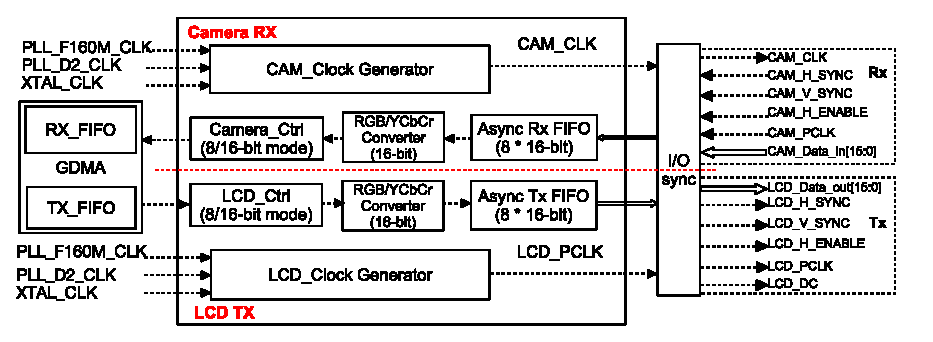
\includegraphics[width=1.0\textwidth]{04-CAMLCDCTRL/figures/i2s-arch_20220617.eps}}
     \textcolor{black}{\textbf{- ->}}：控制信号
     \textcolor{black}{\textbf{=>}}：数据流
    \caption{LCD\_CAM 功能框图}
    \label{Figure:lcdcam_arch}
\end{figure}

\subsection{信号描述}

\begin{ThreePartTable}

\begin{TableNotes}
    \item[1] LCD\_CAM 的所有信号均需要经过 GPIO 交换矩阵映射到芯片管脚。更多信息请参考章节 \ref{mod:iomuxgpio} \textit{\nameref{mod:iomuxgpio}}。
    \item[2] 信号位宽 8 或 16 时，则 \textcolor{red}{\it{N}} 分别为 7 或 15。
    \item[3] \hyperref[fielddesc:LCDCAMCAMVHDEMODEEN]{LCD\_CAM\_CAM\_VH\_DE\_MODE\_EN} 为 1（VSYNC + HSYNC 模式）时：VSYNC、HSYNC、DE 线同时控制数据有效，因此用户需要接 VSYNC、HSYNC、DE 信号线；
\hyperref[fielddesc:LCDCAMCAMVHDEMODEEN]{LCD\_CAM\_CAM\_VH\_DE\_MODE\_EN} 为 0（DE 模式）时：VSYNC、DE 线同时控制数据有效，HSYNC 线可以不接。但是在此模式下，Camera 的 YUV-RGB 转换功能将不可用。
\end{TableNotes}

\begin{longtable}[c]{ | p{3.2cm} | l | c | p{8cm} | }
    \caption{信号描述}
    \label{tab:signal-description}\\\hline

    \rowcolor{lightgray}
    \textbf{工作模式} & \textbf{信号\tnote{1}} & \textbf{方向} & \textbf{功能} \\\hline
    \endfirsthead

    \multicolumn{4}{c}{\bfseries \tablename\ \thetable{} -- 接上页}\\\hline
    \rowcolor{lightgray}
    \textbf{工作模式} & \textbf{信号\tnote{1}} & \textbf{方向} & \textbf{功能} \\\hline
    \endhead

    \multicolumn{4}{r}{\textbf{见下页}} \\
    \endfoot

    \insertTableNotes
    \endlastfoot

    % table contents
    \multirow{5}*{Camera 从机接收模式} & CAM\_PCLK & 输入 & 像素时钟输入信号\\\cline{2-4}
    & CAM\_V\_SYNC & 输入& 帧同步输入信号 (VSYNC)\tnote{3}\\\cline{2-4}
    & CAM\_H\_SYNC & 输入& 行同步输入信号 (HSYNC)\tnote{3}\\\cline{2-4}
    & CAM\_H\_ENABLE & 输入 & 行有效输入信号 (DE)\tnote{3}\\\cline{2-4}
    & CAM\_Data\_in[\textcolor{red}{\it{N}}:0]\tnote{2} & 输入 & 并行输入数据总线，支持 8/16 位并行数据输入\\\hline
    \multirow{6}*{Camera 主机接收模式} & CAM\_PCLK & 输入 & 像素时钟输入信号\\\cline{2-4}
    & CAM\_CLK & 输出& 主机时钟输出信号\\\cline{2-4}
    & CAM\_V\_SYNC & 输入& 帧同步输入信号\tnote{3}\\\cline{2-4}
    & CAM\_H\_SYNC & 输入& 行同步输入信号\tnote{3}\\\cline{2-4}
    & CAM\_H\_ENABLE & 输入 & 行有效输入信号\tnote{3} \\\cline{2-4}
    & CAM\_Data\_in[\textcolor{red}{\it{N}}:0]\tnote{2} & 输入 & 并行输入数据总线，支持 8/16 位并行数据输入\\\hline
    \multirow{7}*{LCD 主机发送模式} & LCD\_PCLK & 输出 & LCD 像素时钟输出信号 \\\cline{2-4}
    & LCD\_H\_SYNC & 输出& RGB 格式下，用作行同步信号  \\\cline{2-4}
    & LCD\_V\_SYNC & 输出 & RGB 格式下，用作帧同步信号 \\\cline{2-4}
    & LCD\_H\_ENABLE & 输出 & RGB 格式下，用作行有效信号 \\\cline{2-4}
    & LCD\_CD & 输出 & I8080 格式下，用作命令和数据信号 (CD) \\\cline{2-4}
    & LCD\_CS & 输出 & I8080/MOTO6800 格式下，用作片选信号 (CS) \\\cline{2-4}
    & LCD\_Data\_out[\textcolor{red}{\it{N}}:0]\tnote{2} & 输出 & 并行输出数据总线，支持 8/16 位并行数据输出\\\hline
\end{longtable}

\end{ThreePartTable}



\subsection{LCD\_CAM 模块时钟}\label{sec:lcdcam-module-clk}

\subsubsection{LCD 时钟}

时钟源经时钟生成模块处理后，生成 LCD 模块所需的时钟，如图 \ref{Figure:lcd_clk} 所示。

其中，
\begin{itemize}
    \item LCD\_CLK 为 LCD 模块的主时钟，由时钟源分频获得；
    \item 像素时钟 LCD\_PCLK 再由 LCD\_CLK 分频获得。
\end{itemize}

寄存器 \hyperref[regdesc:LCDCAMLCDCLOCKREG]{LCD\_CAM\_LCD\_CLOCK\_REG} 中 \hyperref[fielddesc:LCDCAMLCDCLKSEL]{LCD\_CAM\_LCD\_CLK\_SEL} 用于选择时钟源：
\begin{itemize}
    \item 0：关闭 LCD 时钟源；
    \item 1：选择 XTAL\_CLK；
    \item 2：选择 PLL\_D2\_CLK；
    \item 3：选择 PLL\_F160M\_CLK。
\end{itemize}

\begin{figure}[H]
    \centering
    \fbox{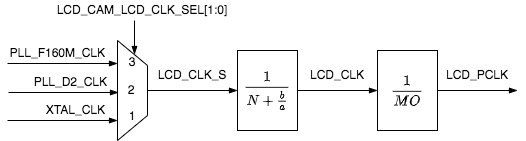
\includegraphics[width=0.8\textwidth]{04-CAMLCDCTRL/figures/lcd_clock_20220617.png}}
    \caption{LCD 时钟}
    \label{Figure:lcd_clk}
\end{figure}


LCD\_CLK 的频率 $f_{\textrm{LCD\_CLK}}$ 与分频器时钟源频率 $f_{\textrm{LCD\_CLK\_S}}$ 间的关系如下：
$$f_{\textrm{LCD\_CLK}}=\frac{f_{\textrm{LCD\_CLK\_S}}}{\textrm{N} + \frac{\textrm{b}}{\textrm{a}}}$$

其中，2 <= N <= 256，N 对应为 \hyperref[regdesc:LCDCAMLCDCLOCKREG]{LCD\_CAM\_LCD\_CLOCK\_REG} 寄存器中 \hyperref[fielddesc:LCDCAMLCDCLKMDIVNUM]{LCD\_CAM\_LCD\_CLKM\_DIV\_NUM} 的值，具体为：

\begin{itemize}
    \item \hyperref[fielddesc:LCDCAMLCDCLKMDIVNUM]{LCD\_CAM\_LCD\_CLKM\_DIV\_NUM} = 0 时，N = 256；
    \item \hyperref[fielddesc:LCDCAMLCDCLKMDIVNUM]{LCD\_CAM\_LCD\_CLKM\_DIV\_NUM} = 1 时，N = 2；
    \item \hyperref[fielddesc:LCDCAMLCDCLKMDIVNUM]{LCD\_CAM\_LCD\_CLKM\_DIV\_NUM} 为其它值时，N = \hyperref[fielddesc:LCDCAMLCDCLKMDIVNUM]{LCD\_CAM\_LCD\_CLKM\_DIV\_NUM} 的值。

\end{itemize}

b 对应 \hyperref[fielddesc:LCDCAMLCDCLKMDIVB]{LCD\_CAM\_LCD\_CLKM\_DIV\_B} 的值，a 对应 \hyperref[fielddesc:LCDCAMLCDCLKMDIVA]{LCD\_CAM\_LCD\_CLKM\_DIV\_A} 的值。对于整数分频，\hyperref[fielddesc:LCDCAMLCDCLKMDIVA]{LCD\_CAM\\\_LCD\_CLKM\_DIV\_A} 和 \hyperref[fielddesc:LCDCAMLCDCLKMDIVB]{LCD\_CAM\_LCD\_CLKM\_DIV\_B} 都清零；对于小数分频，\hyperref[fielddesc:LCDCAMLCDCLKMDIVB]{LCD\_CAM\_LCD\_CLKM\_DIV\_B} 的值应小于 \hyperref[fielddesc:LCDCAMLCDCLKMDIVA]{LCD\_CAM\_LCD\_CLKM\_DIV\_A} 的值。


LCD 模块的像素时钟 PCLK 为 LCD\_PCLK 信号，由 LCD\_CLK 分频获得。即：

$$f_{\textrm{LCD\_PCLK}} = \frac{f_{\textrm{LCD\_CLK}}}{\textrm{MO}}$$


其中，MO 由 \hyperref[fielddesc:LCDCAMLCDCLKEQUSYSCLK]{LCD\_CAM\_LCD\_CLK\_EQU\_SYSCLK} 和 \hyperref[fielddesc:LCDCAMLCDCLKCNTN]{LCD\_CAM\_LCD\_CLKCNT\_N} 决定，具体为：

\begin{itemize}
    \item \hyperref[fielddesc:LCDCAMLCDCLKEQUSYSCLK]{LCD\_CAM\_LCD\_CLK\_EQU\_SYSCLK} = 1 时，MO = 1；
    \item \hyperref[fielddesc:LCDCAMLCDCLKEQUSYSCLK]{LCD\_CAM\_LCD\_CLK\_EQU\_SYSCLK} = 0 时，MO = \hyperref[fielddesc:LCDCAMLCDCLKCNTN]{LCD\_CAM\_LCD\_CLKCNT\_N} + 1。
\end{itemize}

{\bfseries 注意：}
\begin{itemize}
    \item \hyperref[fielddesc:LCDCAMLCDCLKCNTN]{LCD\_CAM\_LCD\_CLKCNT\_N} 不可配置为 0；
    \item 使用小数分频功能会产生时钟抖动。当 LCD\_CLK 和 LCD\_PCLK 无法通过 PLL\_F160M\_CLK 整数分频产生时，可使用 PLL\_D2\_CLK 作为时钟源，详情请参考章节 \ref{mod:resclk} \textit{\nameref{mod:resclk}}。
\end{itemize}

\subsubsection{Camera 时钟}

时钟源经时钟生成模块处理后，生成 Camera 模块所需的时钟，如图 \ref{Figure:camera_clk} 所示。

其中，
\begin{itemize}
    \item CAM\_CLK 为 Camera 模块的主机时钟输出，由时钟源分频获得；
    \item 像素时钟 LCD\_PCLK 由 Camera 从机输入获得。
\end{itemize}

寄存器 \hyperref[regdesc:LCDCAMCAMCTRLREG]{LCD\_CAM\_CAM\_CTRL\_REG} 中 \hyperref[fielddesc:LCDCAMCAMCLKSEL]{LCD\_CAM\_CAM\_CLK\_SEL} 用于选择时钟源：
\begin{itemize}
    \item 0：关闭 CAM 时钟源；
    \item 1：选择 XTAL\_CLK；
    \item 2：选择 PLL\_D2\_CLK；
    \item 3：选择 PLL\_F160M\_CLK。
\end{itemize}


\begin{figure}[H]
    \centering
    \fbox{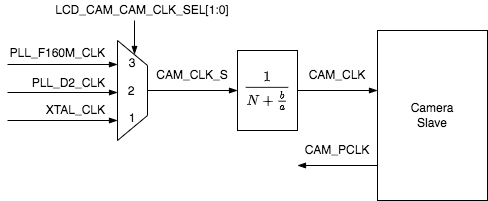
\includegraphics[width=0.8\textwidth]{04-CAMLCDCTRL/figures/camera_clock_20220617.png}}
    \caption{Camera 时钟}
    \label{Figure:camera_clk}
\end{figure}

CAM\_CLK 的频率 $f_{\textrm{CAM\_CLK}}$ 与分频器时钟源频率 $f_{\textrm{CAM\_CLK\_S}}$ 间的关系如下：
$$f_{\textrm{CAM\_CLK}}=\frac{f_{\textrm{CAM\_CLK\_S}}}{\textrm{N} + \frac{\textrm{b}}{\textrm{a}}}$$

其中，2 <= N <= 256，N 对应为 \hyperref[regdesc:LCDCAMCAMCTRLREG]{LCD\_CAM\_CAM\_CTRL\_REG} 寄存器中 \hyperref[fielddesc:LCDCAMCAMCLKMDIVNUM]{LCD\_CAM\_CAM\_CLKM\_DIV\_NUM} 的值，具体为：

\begin{itemize}
    \item \hyperref[fielddesc:LCDCAMCAMCLKMDIVNUM]{LCD\_CAM\_CAM\_CLKM\_DIV\_NUM} = 0 时，N = 256；
    \item \hyperref[fielddesc:LCDCAMCAMCLKMDIVNUM]{LCD\_CAM\_CAM\_CLKM\_DIV\_NUM} = 1 时，N = 2；
    \item \hyperref[fielddesc:LCDCAMCAMCLKMDIVNUM]{LCD\_CAM\_CAM\_CLKM\_DIV\_NUM} 为其它值时，N = \hyperref[fielddesc:LCDCAMCAMCLKMDIVNUM]{LCD\_CAM\_CAM\_CLKM\_DIV\_NUM} 的值。

\end{itemize}

b 对应 \hyperref[fielddesc:LCDCAMCAMCLKMDIVB]{LCD\_CAM\_CAM\_CLKM\_DIV\_B} 的值，a 对应 \hyperref[fielddesc:LCDCAMCAMCLKMDIVA]{LCD\_CAM\_CAM\_CLKM\_DIV\_A} 的值。对于整数分频，\hyperref[fielddesc:LCDCAMCAMCLKMDIVA]{LCD\_CAM\\\_CAM\_CLKM\_DIV\_A} 和 \hyperref[fielddesc:LCDCAMCAMCLKMDIVB]{LCD\_CAM\_CAM\_CLKM\_DIV\_B} 都清零；对于小数分频，\hyperref[fielddesc:LCDCAMCAMCLKMDIVB]{LCD\_CAM\_CAM\_CLKM\_DIV\_B} 的值应小于 \hyperref[fielddesc:LCDCAMCAMCLKMDIVA]{LCD\_CAM\_CAM\_CLKM\_DIV\_A} 的值。



\subsection{LCD\_CAM 模块复位} \label{module_reset}
LCD\_CAM 模块中各个单元可通过配置下列寄存器进行复位：
\begin{itemize}
\item 发送控制单元 (LCD\_Ctrl) 及其格式转换模块 (RGB/YCbCr Converter)：可配置 \hyperref[fielddesc:LCDCAMLCDRESET]{LCD\_CAM\_LCD\_RESET} 进行复位；
\item 接收控制单元 (Camera\_Ctrl) 及其格式转换模块 (RGB/YCbCr Converter)：可配置 \hyperref[fielddesc:LCDCAMCAMRESET]{LCD\_CAM\_CAM\_RESET} 进行复位；
\item Async Tx FIFO：可配置 \hyperref[fielddesc:LCDCAMLCDAFIFORESET]{LCD\_CAM\_LCD\_AFIFO\_RESET} 进行复位；
\item Async Rx FIFO：可配置 \hyperref[fielddesc:LCDCAMCAMAFIFORESET]{LCD\_CAM\_CAM\_AFIFO\_RESET} 进行复位。
\end{itemize}


{\bfseries 注意：}
\begin{itemize}
    \item 上述复位寄存器均为硬件自清，即写 1 后，硬件会自动清零；
    \item 在模块和 FIFO 复位之前，需要先配置 LCD 或 Camera 模块时钟。
\end{itemize}

\subsection{LCD\_CAM 数据格式控制}
\subsubsection{LCD 数据格式控制} \label{lcd_data_control}
在使用 LCD 发送数据时，配置以下寄存器可以调整来自 DMA 的数据的比特/字节序：

\begin{itemize}
    \item \hyperref[fielddesc:LCDCAMLCD2BYTEEN]{LCD\_CAM\_LCD\_2BYTE\_EN}
    \begin{itemize}
        \item 1：：LCD 输出的数据位宽为 16 个比特；
        \item 0：LCD 输出的数据位宽为 8 个比特。
    \end{itemize}
    \item \hyperref[fielddesc:LCDCAMLCDBITORDER]{LCD\_CAM\_LCD\_BIT\_ORDER}
    \begin{itemize}
        \item 反转数据位顺序：
        \begin{itemize}
            \item 在 8-bit 模式下，LCD\_DATA\_out[7:0] 反转为 LCD\_DATA\_out[0:7]；
            \item 在 16-bit 模式下，LCD\_DATA\_out[15:0] 反转为 LCD\_DATA\_out[0:15]。
        \end{itemize}
        \item 不反转。
    \end{itemize}
    \item \hyperref[fielddesc:LCDCAMLCDBYTEORDER]{LCD\_CAM\_LCD\_BYTE\_ORDER}
    \begin{itemize}
        \item 1：反转数据字节顺序。仅在 16-bit 模式下有效；
        \item 0：不反转。
    \end{itemize}
    \item \hyperref[fielddesc:LCDCAMLCD8BITSORDER]{LCD\_CAM\_LCD\_8BITS\_ORDER}
    \begin{itemize}
        \item 1：两个字节反转位置。仅在 8-bit 模式下有效；
        \item 0：不反转。
    \end{itemize}
\end{itemize}

具体配置方式见下表。

\begin{table}[H]
    \centering
    \caption{LCD 数据格式控制}
    \label{tab:bit-byte-order-control-of-lcd-data}
    \begin{threeparttable}
    \begin{tabular}{|p{2.3cm}|p{2.4cm}|p{2.5cm}|p{2.5cm}|p{2.6cm}|p{3.1cm}|}
    \hline
    \rowcolor{lightgray}
    \textbf{DMA 数据序列\tnote{1}} & \textbf{\hyperref[fielddesc:LCDCAMLCD2BYTEEN]{LCD\_CAM\_LCD\newline\_2BYTE\_EN}}  & \textbf{\hyperref[fielddesc:LCDCAMLCDBITORDER]{LCD\_CAM\_LCD\newline\_BIT\_ORDER}}  & \textbf{\hyperref[fielddesc:LCDCAMLCDBYTEORDER]{LCD\_CAM\_LCD\newline\_BYTE\_ORDER}\tnote{2}} &  \textbf{\hyperref[fielddesc:LCDCAMLCD8BITSORDER]{LCD\_CAM\_LCD\newline\_8BITS\_ORDER}\tnote{2}} & \textbf{发送数据序列\tnote{3,4}}
    \\ \hline
    \multirow{8}*{B0,B1,B2,B3} & \multirow{4}*{0} & \multirow{2}*{0} & 0 & 0 & \{B0\}\{B1\}\{B2\}\{B3\}     \\\cline{4-6}
                               &                  &                  & 0 & 1 & \{B1\}\{B0\}\{B3\}\{B2\}     \\\cline{3-6}
                               &                  & \multirow{2}*{1} & 0 & 0 & \{B0'\}\{B1'\}\{B2'\}\{B3'\} \\\cline{4-6}
                               &                  &                  & 0 & 1 & \{B1'\}\{B0'\}\{B3'\}\{B2'\} \\\cline{2-6}
                               & \multirow{4}*{1} & \multirow{2}*{0} & 0 & 0 & \{B1,B0\}\{B3,B2\}           \\\cline{4-6}
                               &                  &                  & 1 & 0 & \{B0,B1\}\{B2,B3\}           \\\cline{3-6}
                               &                  & \multirow{2}*{1} & 0 & 0 & \{B1',B0'\}\{B3',B2'\}       \\\cline{4-6}
                               &                  &                  & 1 & 0 & \{B0',B1'\}\{B2',B3'\}       \\\hline
    \end{tabular}
    \begin{tablenotes}
        \item[1] DMA 数据序列中的 B0 \verb+~+ B3 每一个代表一个字节的数据，靠左的数据对应低地址，即 B0 \verb+~+ B3 的地址为从低到高。
        \item[2] 只有表格中的配置组合是有效的，所有表格所示之外的配置组合可能会导致不可预期的数据错误。
        \item[3] 发送数据序列中，每个 \{\} 中的数据为大端并行数据，各个 \{\} 中的数据为串行关系，发送顺序为从左至右。以 \{B0\}\{B1\}\{B2\}\{B3\} 为例，\{B0\} 中的各个数据位之间为并行关系，而 \{B0\} 中的数据与 \{B1\}、\{B2\}、\{B3\} 的数据为串行关系。发送顺序为先发送 \{B0\}。
        \item[4] 发送数据序列中，B{\textcolor{red}{n}}'[7:0] = B{\textcolor{red}{n}}[0:7]，其中 n = 0,1,2,3。
    \end{tablenotes}
    \end{threeparttable}
\end{table}

\begin{tiplisting}
注意：当发送序列为每次发送 1 个字节数据时，LCD\_Data\_out[7:0] 为有效数据，LCD\_Data\_out[15:8] 为无效数据。
\end{tiplisting}

\subsubsection{Camera 数据格式控制} \label{cam_data_control}
在使用 Camera 接收数据时，配置以下寄存器可以调整送往 DMA 的数据的比特/字节序：
\begin{itemize}
    \item \hyperref[fielddesc:LCDCAMCAM2BYTEEN]{LCD\_CAM\_CAM\_2BYTE\_EN}
    \begin{itemize}
        \item 1：接收数据的位宽为 16 个比特；
        \item 0：接收数据的位宽为 8 个比特。
    \end{itemize}
    \item \hyperref[fielddesc:LCDCAMCAMBITORDER]{LCD\_CAM\_CAM\_BIT\_ORDER}
    \begin{itemize}
        \item 1：反转数据位顺序：
        \begin{itemize}
            \item 在 8-bit 模式下，CAM\_DATA\_in[7:0] 反转为 CAM\_DATA\_in[0:7]；
            \item 在 16-bit 模式下，CAM\_DATA\_in[15:0] 反转为 CAM\_DATA\_in[0:15]。
        \end{itemize}
        \item 0：不反转。
    \end{itemize}
    \item \hyperref[fielddesc:LCDCAMCAMBYTEORDER]{LCD\_CAM\_CAM\_BYTE\_ORDER}
    \begin{itemize}
        \item 1：反转数据字节顺序。仅在 16-bit 模式下有效；
        \item 0：不反转。
    \end{itemize}
\end{itemize}

具体配置方式见下表。

\begin{table}[H]
    \centering
    \caption{Camera 数据格式控制}
    \label{tab:bit-byte-order-control-of-cam-data}
    \begin{threeparttable}
    \begin{tabular}{|p{2.7cm}|p{2.6cm}|p{2.6cm}|p{2.6cm}|p{2.7cm}|}
    \hline
    \rowcolor{lightgray}
    \textbf{接收数据序列\tnote{1}} & \textbf{\hyperref[fielddesc:LCDCAMCAM2BYTEEN]{LCD\_CAM\_CAM\newline\_2BYTE\_EN}}  & \textbf{\hyperref[fielddesc:LCDCAMCAMBITORDER]{LCD\_CAM\_CAM\newline\_BIT\_ORDER}\tnote{2}}  & \textbf{\hyperref[fielddesc:LCDCAMCAMBYTEORDER]{LCD\_CAM\_CAM\newline\_BYTE\_ORDER}\tnote{2}} & \textbf{DMA 数据序列\tnote{3,4}}
    \\ \hline
    \multirow{2}*{\{B0\}\{B1\}\{B2\}\{B3\}} & \multirow{2}*{0} &        0         & 0 & B0,B1,B2,B3     \\\cline{3-5}
                                            &                  &        1         & 0 & B0',B1',B2',B3' \\\hline
    \multirow{4}*{\{B1,B0\}\{B3,B2\}}       & \multirow{4}*{1} & \multirow{2}*{0} & 0 & B0,B1,B2,B3     \\\cline{4-5}
                                            &                  &                  & 1 & B1,B0,B3,B2     \\\cline{3-5}
                                            &                  & \multirow{2}*{1} & 0 & B0',B1',B2',B3' \\\cline{4-5}
                                            &                  &                  & 1 & B1',B0',B3',B2' \\\hline
    \end{tabular}
    \begin{tablenotes}
        \item[1] 接收数据序列中，每个 \{\} 中的数据为大端并行数据，各个 \{\} 中的数据为串行关系，接收顺序为从左至右。以 \{B0\}\{B1\}\{B2\}\{B3\} 为例，\{B0\} 中的各个数据位之间为并行关系，而 \{B0\} 中的数据与 \{B1\}、\{B2\}、\{B3\} 的数据为串行关系。接收顺序为先接收 \{B0\}。
        \item[2] 只有表格中的配置组合是有效的，所有表格所示之外的配置组合可能会导致不可预期的数据错误。
        \item[3] DMA 数据序列中的 B0 \verb+~+ B3 每一个代表一个字节的数据，靠左的数据对应低地址，即 B0 \verb+~+ B3 的地址为从低到高。
        \item[4] DMA 数据序列中，B{\textcolor{red}{n}}'[7:0] = B{\textcolor{red}{n}}[0:7]，其中 n = 0,1,2,3。
    \end{tablenotes}
    \end{threeparttable}
\end{table}

\begin{tiplisting}
注意：当接收序列为每次接收 1 个字节数据时，CAM\_Data\_in[7:0] 为有效数据，因此用户需要将 CAM\_Data\_in[7:0] 与主机相连。
\end{tiplisting}

\subsection{YUV-RGB 数据格式转换}
\chipname{} LCD\_CAM 模块支持 YUV-RGB 数据格式互相转换。LCD 模块以及 Camera 模块各有一个数据格式转换模块，其功能包括：
\begin{itemize}
    \item 支持在 BT601 和 BT709 两种标准下进行格式转换；
    \item RGB565 (full/limited range) 格式与 YUV422/420/411 (full/limited range) 格式的互相转换；
    \item YUV422/420/411 (full/limited range) 各种格式的互相转换。
\end{itemize}

\subsubsection{YUV 时序}
在 \chipname{} LCD\_CAM 模块中我们作以下规定：

假设 8 个依次待传输像素点对应的 YUV 数据为 [$Y_i$, $U_i$, $V_i$] (i = 1 \verb+~+ 8)，则在：
\begin{itemize}
    \item YUV422 模式下，LCD 依次发送或 Camera 依次接收如下数据：
        \begin{table}[H]
            \centering
            \begin{tabular}{|c|c|c|c|c|c|c|c|c|c|c|c|c|c|c|c|}
            \hline
            $Y_1$ & $U_1$ & $Y_2$ & $V_2$ & $Y_3$ & $U_3$ & $Y_4$ & $V_4$ & $Y_5$ & $U_5$ & $Y_6$ & $V_6$ & $Y_7$ & $U_7$ & $Y_8$ & $V_8$ \\ \hline
            \end{tabular}
        \end{table}
    \item YUV420 模式下，LCD 依次发送或 Camera 依次接收如下数据：
        \begin{table}[H]
            \centering
            \begin{tabular}{|c|c|c|c|c|c|c|c|c|c|c|c|}
            \hline
            $Y_1$ & $U_1$ & $Y_2$ & $Y_3$ & $U_3$ & $Y_4$ & $Y_5$ & $V_5$ & $Y_6$ & $Y_7$ & $V_7$ & $Y_8$ \\ \hline
            \end{tabular}
        \end{table}
    \item YUV411 模式下，LCD 依次发送或 Camera 依次接收如下数据：
        \begin{table}[H]
            \centering
            \begin{tabular}{|c|c|c|c|c|c|c|c|c|c|c|c|}
            \hline
            $Y_1$ & $U_1$ & $Y_2$ & $Y_3$ & $V_3$ & $Y_4$ & $Y_5$ & $U_5$ & $Y_6$ & $Y_7$ & $V_7$ & $Y_8$ \\ \hline
            \end{tabular}
        \end{table}
\end{itemize}

\subsubsection{格式转换模块配置流程}
Camera 模块中的格式转换模块与 LCD 模块中的格式转换模块完全相同。因此，下文以 LCD 模块中的格式转换模块为例说明配置流程：
\begin{itemize}
    \item 使能 YUV-RGB 格式转换模块：置位 \hyperref[fielddesc:LCDCAMLCDCONVBYPASS]{LCD\_CAM\_LCD\_CONV\_BYPASS}；
    \item 配置数据传输模式：配置 \hyperref[fielddesc:LCDCAMLCDCONVMODE8BITSON]{LCD\_CAM\_LCD\_CONV\_MODE\_8BITS\_ON} 为：
    \begin{itemize}
        \item 0：使用 16 线数据传输模式
        \item 1：使用 8 线数据传输模式
    \end{itemize}
    \item 配置标准：配置 \hyperref[fielddesc:LCDCAMLCDCONVPROTOCOLMODE]{LCD\_CAM\_LCD\_CONV\_PROTOCOL\_MODE} 为：
    \begin{itemize}
        \item 0：使用 BT601 标准
        \item 1：使用 BT709 标准
    \end{itemize}
    \item 配置转换模式：
        \begin{table}[H]
        \caption{转换模式配置}
        \centering
        \begin{threeparttable}
        \begin{tabular}{|l|c|c|c|}
        \hline
        \rowcolor{lightgray}
        \textbf{转换模式} & \textbf{\hyperref[fielddesc:LCDCAMLCDCONVTRANSMODE]{TRANS\_MODE}}\tnote{1} & \textbf{\hyperref[fielddesc:LCDCAMLCDCONVYUVMODE]{YUV\_MODE}}\tnote{2} & \textbf{\hyperref[fielddesc:LCDCAMLCDCONVYUV2YUVMODE]{YUV2YUV\_MODE}}\tnote{3} \\ \hline
        RGB565 -> YUV422 & 1 & 0 & 3 \\ \hline
        RGB565 -> YUV420 & 1 & 1 & 3 \\ \hline
        RGB565 -> YUV411 & 1 & 2 & 3 \\ \hline
        YUV422 -> RGB565 & 0 & 0 & 3 \\ \hline
        YUV420 -> RGB565 & 0 & 1 & 3 \\ \hline
        YUV411 -> RGB565 & 0 & 2 & 3 \\ \hline
        YUV422 -> YUV420 & 1 & 0 & 1 \\ \hline
        YUV422 -> YUV411 & 1 & 0 & 2 \\ \hline
        YUV420 -> YUV422 & 1 & 1 & 0 \\ \hline
        YUV420 -> YUV411 & 1 & 1 & 2 \\ \hline
        YUV411 -> YUV422 & 1 & 2 & 0 \\ \hline
        YUV411 -> YUV420 & 1 & 2 & 1 \\ \hline
        \end{tabular}
        \begin{tablenotes}
            \item[1] 对应 \hyperref[fielddesc:LCDCAMLCDCONVTRANSMODE]{LCD\_CAM\_LCD\_CONV\_TRANS\_MODE} 的值
            \item[2] 对应 \hyperref[fielddesc:LCDCAMLCDCONVTRANSMODE]{LCD\_CAM\_LCD\_CONV\_YUV\_MODE} 的值
            \item[3] 对应 \hyperref[fielddesc:LCDCAMLCDCONVTRANSMODE]{LCD\_CAM\_LCD\_CONV\_YUV2YUV\_MODE} 的值
        \end{tablenotes}
     \end{threeparttable}
    \end{table}

    \item 配置输入数据色彩空间：配置 \hyperref[fielddesc:LCDCAMLCDCONVDATAINMODE]{LCD\_CAM\_LCD\_CONV\_DATA\_IN\_MODE} 为：
    \begin{itemize}
        \item 0：有限色彩空间 (limited range)
        \item 1：全色彩空间 (full range)
    \end{itemize}

    \item 配置输出数据色彩空间：配置 \hyperref[fielddesc:LCDCAMLCDCONVDATAOUTMODE]{LCD\_CAM\_LCD\_CONV\_DATA\_OUT\_MODE} 为：
    \begin{itemize}
        \item 1：全色彩空间 (full range)\hyperref[full-color-range-note]{$^1$}
        \item 0：有限色彩空间 (limited range)\hyperref[limited-color-range-note]{$^2$}
    \end{itemize}
\end{itemize}

\begin{tiplisting}
\vspace{-2em}
\begin{enumerate}
    \item \label{full-color-range-note} 如果选择全色彩空间，则 RGB 或 YUV 的取值范围为：0 \verb+~+ 255；
    \item \label{limited-color-range-note} 如果选择有限色彩空间，则\begin{itemize}
        \item RGB 的取值范围为：16 \verb+~+ 240；
        \item YUV 的取值范围为：
        \begin{itemize}
            \item Y：16 \verb+~+ 240；
            \item U-V：16 \verb+~+ 235。
        \end{itemize}

    \end{itemize}

\end{enumerate}
\end{tiplisting}

\section{软件配置流程}
\begin{tiplisting}
LCD 模块和 Camera 模块的寄存器相关配置，均需要通过置位对应的 \hyperref[fielddesc:LCDCAMLCDUPDATE]{LCD\_CAM\_LCD\_UPDATE} 和 \hyperref[fielddesc:LCDCAMCAMUPDATE]{LCD\_CAM\_CAM\_\\UPDATE} 的方式来进行更新，从而将 LCD 寄存器数据从 APB 时钟域同步到 LCD/Camera 时钟域。见下文示例。
\end{tiplisting}
\vspace{-2em}
\subsection{软件配置 LCD（RGB 格式）发送流程}
软件配置 LCD 以 RGB 格式发送的流程如下：

\begin{enumerate}
    \item 根据 \ref{sec:lcdcam-module-clk} 小节的描述，配置时钟；
    \item 根据表 \ref{tab:signal-description} 的描述，配置信号管脚；

    \item 根据 \ref{LCDCAM_INT} 小节的描述使能相应的中断；\label{LCDCAM-TX-INTERRUPT1}

    \item 置位 \hyperref[fielddesc:LCDCAMLCDRGBMODEEN]{LCD\_CAM\_LCD\_RGB\_MODE\_EN}，使能 RGB 格式；

    \item 配置以下帧格式寄存器，如下图所示：
    \begin{itemize}
        \item \hyperref[fielddesc:LCDCAMLCDVTHEIGHT]{LCD\_CAM\_LCD\_VT\_HEIGHT}
        \item \hyperref[fielddesc:LCDCAMLCDVTHEIGHT]{LCD\_CAM\_LCD\_VA\_HEIGHT}
        \item \hyperref[fielddesc:LCDCAMLCDVTHEIGHT]{LCD\_CAM\_LCD\_HB\_FRONT}
        \item \hyperref[fielddesc:LCDCAMLCDHTWIDTH]{LCD\_CAM\_LCD\_HT\_WIDTH}
        \item \hyperref[fielddesc:LCDCAMLCDHTWIDTH]{LCD\_CAM\_LCD\_HA\_WIDTH}
        \item \hyperref[fielddesc:LCDCAMLCDHTWIDTH]{LCD\_CAM\_VB\_FRONT}
        \item \hyperref[fielddesc:LCDCAMLCDVSYNCWIDTH]{LCD\_CAM\_LCD\_VSYNC\_WIDTH}

    \end{itemize}
\begin{figure}[H]
    \centering
    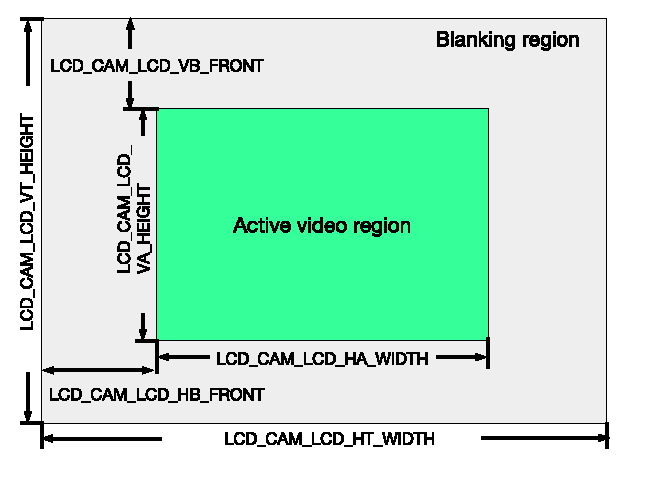
\includegraphics[width=0.6\textwidth]{04-CAMLCDCTRL/figures/lcd_frame_structure}
    \caption{LCD 视频帧结构}
    \label{fig:lcd_frame}
\end{figure}

\begin{figure}[H]
    \centering
    \fbox{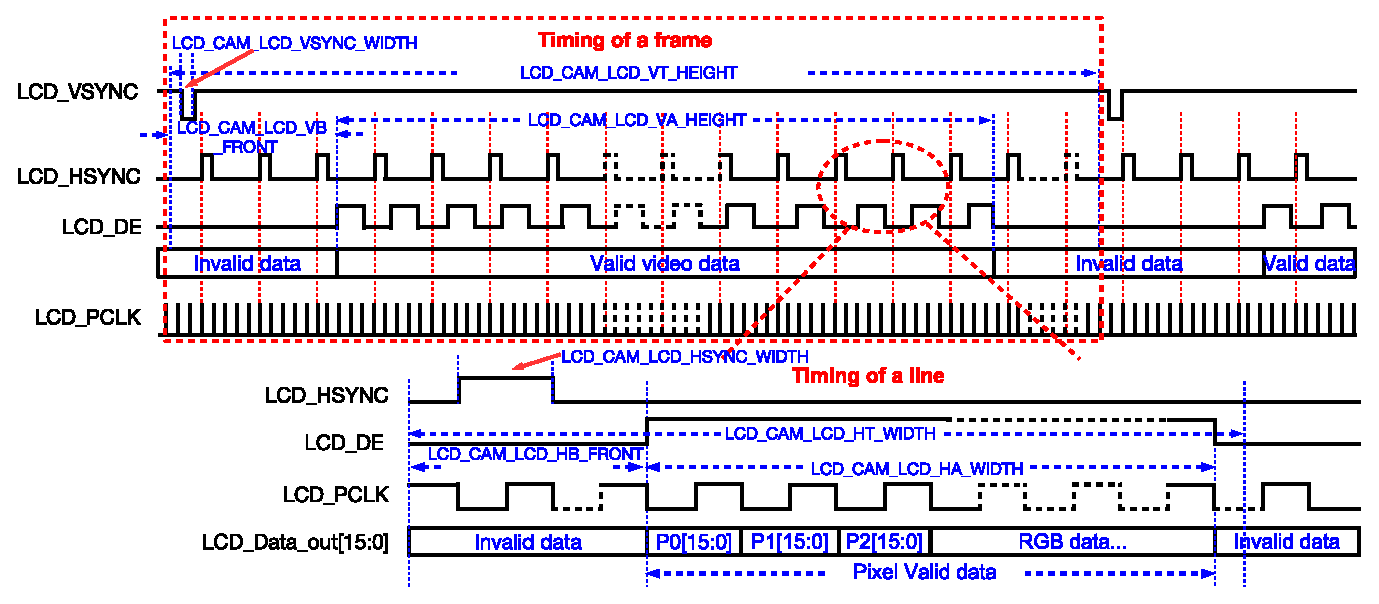
\includegraphics[width=1.0\textwidth]{04-CAMLCDCTRL/figures/lcd_timing_20220216}}
    \caption{LCD 时序（RGB 格式）}
    \label{fig:lcd_timing}
\end{figure}

\begin{tiplisting}
配置上图所示的时序参数时，请特别注意参数与寄存器的关系。参数值等于寄存器值 + 1。例如，如果希望 VSYNC 宽度为 1，则需要配置 \hyperref[fielddesc:LCDCAMLCDVSYNCWIDTH]{LCD\_CAM\_LCD\_VSYNC\_WIDTH} 为 0。更多信息见寄存器描述部分。
\end{tiplisting}

    \item 置位 \hyperref[fielddesc:LCDCAMLCDUPDATE]{LCD\_CAM\_LCD\_UPDATE}；

    \item 根据 \ref{module_reset} 小节的描述，复位发送控制单元 (LCD\_Ctrl) 和 Async Tx FIFO；

    \item 配置 GDMA 发送链表；

    \item 开始发送数据：
    \begin{itemize}
        \item 等待 LCD 从设备配置完成；
        \item 置位 \hyperref[fielddesc:LCDCAMLCDSTART]{LCD\_CAM\_LCD\_START} 开始发送数据。
    \end{itemize}

    \item 等待步骤 \ref{LCDCAM-TX-INTERRUPT1} 设置的中断信号；

    \item 在数据发送的帧间隔，检查 \hyperref[fielddesc:LCDCAMLCDNEXTFRAMEEN]{LCD\_CAM\_LCD\_NEXT\_FRAME\_EN} 是否被置位：
    \begin{itemize}
        \item 如果被置位，则继续发送下一帧数据：置位 \hyperref[fielddesc:LCDCAMLCDUPDATE]{LCD\_CAM\_LCD\_UPDATE}，重复上述步骤；
        \item 如果没有被置位，则 LCD 停止发送数据。
    \end{itemize}

    \item 若数据发送完成，则清零 \hyperref[fielddesc:LCDCAMLCDSTART]{LCD\_CAM\_LCD\_START}。
\end{enumerate}

\subsection{软件配置 LCD（I8080/MOTO6800 格式）发送流程}

图 \ref{fig:lcd_i8080_timing} 所示为 LCD 时序图（I8080 格式）。


\begin{figure}[H]
    \centering
    \fbox{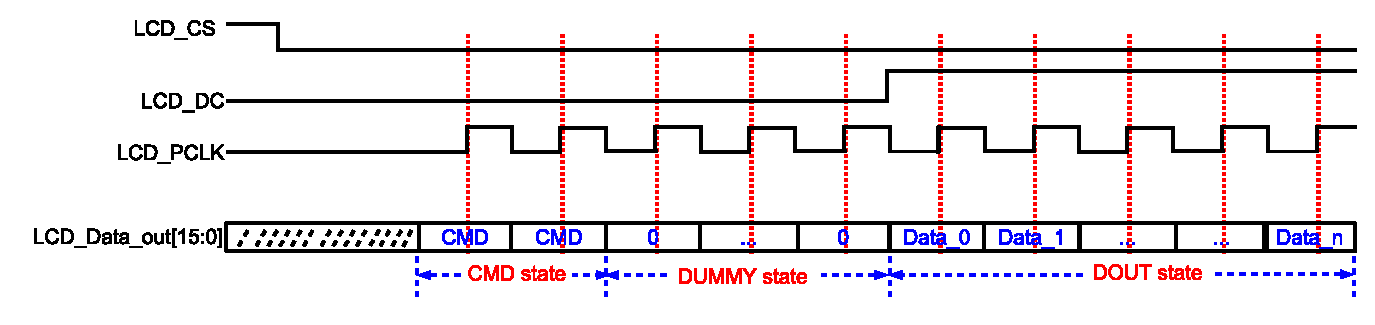
\includegraphics[width=1.0\textwidth]{04-CAMLCDCTRL/figures/LCD_I8080_Timg}}
    \caption{LCD 时序（I8080 格式）}
    \label{fig:lcd_i8080_timing}
\end{figure}

软件配置 LCD 以 I8080 格式发送的流程如下：




\begin{enumerate}
    \item 根据 \ref{sec:lcdcam-module-clk} 小节的描述，配置时钟；

    \item 根据表 \ref{tab:signal-description} 的描述，配置信号管脚；

    \item 根据 \ref{LCDCAM_INT} 小节的描述使能相应的中断；\label{LCDCAM-TX-INTERRUPT}

    \item 清零 \hyperref[fielddesc:LCDCAMLCDRGBMODEEN]{LCD\_CAM\_LCD\_RGB\_MODE\_EN}；
    \item 配置 CMD 阶段，包括 \hyperref[fielddesc:LCDCAMLCDCMD]{LCD\_CAM\_LCD\_CMD}、\hyperref[fielddesc:LCDCAMLCDCMD2CYCLEEN]{LCD\_CAM\_LCD\_CMD\_2\_CYCLE\_EN}、\hyperref[fielddesc:LCDCAMLCDCMDVALUE]{LCD\_CAM\_LCD\_CMD\\\_VALUE}；
    \item 配置 DUMMY 阶段，包括 \hyperref[fielddesc:LCDCAMLCDDUMMY]{LCD\_CAM\_LCD\_DUMMY}、\hyperref[fielddesc:LCDCAMLCDDUMMYCYCLELEN]{LCD\_CAM\_LCD\_DUMMY\_CYCLELEN}；
    \item 配置 DOUT 阶段，包括 \hyperref[fielddesc:LCDCAMLCDDOUT]{LCD\_CAM\_LCD\_DOUT}，根据输出模式不同进行以下配置：
\begin{itemize}
    \item 定长输出模式\hyperref[note-1]{$^a$}，在 \hyperref[fielddesc:LCDCAMLCDDOUTCYCLELEN]{LCD\_CAM\_LCD\_DOUT\_CYCLELEN} 中配置数据长度；
    \item 持续输出模式\hyperref[note-2]{$^b$}，则需：


    \begin{itemize}
        \item 置位 \hyperref[fielddesc:LCDCAMLCDALWAYSOUTEN]{LCD\_CAM\_LCD\_ALWAYS\_OUT\_EN} 使能持续输出模式；
        \item 不需要配置 \hyperref[fielddesc:LCDCAMLCDDOUTCYCLELEN]{LCD\_CAM\_LCD\_DOUT\_CYCLELEN}。
    \end{itemize}

\begin{tiplisting}
\vspace{-2em}
\begin{enumerate}
    \item \label{note-1} 定长输出模式是指：LCD 发送完成 \hyperref[fielddesc:LCDCAMLCDDOUTCYCLELEN]{LCD\_CAM\_LCD\_DOUT\_CYCLELEN} 中配置的数据长度即结束 LCD 发送。
    \item \label{note-2} 持续输出模式是指：LCD 持续发送数据，直到
    \begin{enumerate}
        \item \hyperref[fielddesc:LCDCAMLCDSTART]{LCD\_CAM\_LCD\_START} 被清零；
        \item \hyperref[fielddesc:LCDCAMLCDRESET]{LCD\_CAM\_LCD\_RESET} 被置位；
        \item GDMA 中所有数据被发送完。
    \end{enumerate}
\end{enumerate}
\end{tiplisting}
\end{itemize}
    \item 配置 CD 信号模式，包括 CD 信号的默认值以及在各阶段的值，详见寄存器 \hyperref[regdesc:LCDCAMLCDMISCREG]{LCD\_CAM\_LCD\_MISC\_REG} 描述；

    \item 置位 \hyperref[fielddesc:LCDCAMLCDUPDATE]{LCD\_CAM\_LCD\_UPDATE}；

    \item 根据 \ref{module_reset} 小节的描述，复位发送控制单元 (LCD\_Ctrl) 和 Async Tx FIFO；

    \item 配置 GDMA 发送链表；

    \item 开始发送数据：
    \begin{itemize}
        \item 等待 LCD 从设备配置完成；
        \item 置位 \hyperref[fielddesc:LCDCAMLCDSTART]{LCD\_CAM\_LCD\_START} 开始发送数据。
    \end{itemize}

    \item 等待步骤 \ref{LCDCAM-TX-INTERRUPT} 设置的中断信号；

    \item 若数据发送完成，则清零 \hyperref[fielddesc:LCDCAMLCDSTART]{LCD\_CAM\_LCD\_START}。
\end{enumerate}

\textbf{注意：}\\
无论 LCD 配置为 RGB 格式，还是 I8080/MOTO6800 格式，访问内部存储器时均应注意以下限制：
\begin{itemize}
    \item 如果 LCD 数据总线设置为 8-bit 并行输出时，则
    \begin{itemize}
        \item 像素时钟频率需小于 80 MHz；
        \item 如果同时使用了 YUV-RGB 格式转换，则像素时钟频率需小于 60 MHz。
    \end{itemize}
    \item 如果 LCD 数据总线设置为 16-bit 并行输出时，则
    \begin{itemize}
        \item 像素时钟频率需小于 40 MHz；
        \item 如果同时使用了 YUV-RGB 格式转换，则像素时钟频率需小于 30 MHz。
    \end{itemize}
\end{itemize}




\subsection{软件配置 Camera 接收流程}
软件配置 Camera 接收模式的流程如下：

\begin{enumerate}
    \item 根据 \ref{sec:lcdcam-module-clk} 小节的描述，配置时钟。注意，在从机模式下，模块时钟频率需要大于 2 倍的图形传感器的 PCLK 频率；

    \item 根据表 \ref{tab:signal-description} 的描述，配置信号管脚；

    \item 根据控制信号 HSYNC 是否有效置位或清零 \hyperref[fielddesc:LCDCAMCAMVHDEMODEEN]{LCD\_CAM\_CAM\_VH\_DE\_MODE\_EN}；
    \item 配置正确的接收通道模式和接收数据模式，置位 \hyperref[fielddesc:LCDCAMCAMUPDATE]{LCD\_CAM\_CAM\_UPDATE}；

    \item 根据 \ref{module_reset} 小节的描述，复位接收控制单元 (Camera\_Ctrl) 和 Async Rx FIFO；
    \item 根据 \ref{LCDCAM_INT} 小节的描述使能相应的中断；\label{LCDCAM-RX-INTERRUPT}

    \item 配置 GDMA 接收链表，并在 \hyperref[fielddesc:LCDCAMCAMRECDATABYTELEN]{LCD\_CAM\_CAM\_REC\_DATA\_BYTELEN} 中配置接收数据长度；

    \item 开始接收数据：
    \begin{itemize}
        \item 在主机模式下，等待从机准备好后，置位 \hyperref[fielddesc:LCDCAMCAMSTART]{LCD\_CAM\_CAM\_START} 开始接收数据；
        \item 在从机模式下，置位 \hyperref[fielddesc:LCDCAMCAMSTART]{LCD\_CAM\_CAM\_START}，等待主机提供时钟和控制信号后开始接收数据。
    \end{itemize}
    \item 接收数据，并存到 \chipname{}  存储器的指定地址。最终产生步骤 \ref{LCDCAM-RX-INTERRUPT} 中设置的中断。
\end{enumerate}

\textbf{注意：}
\begin{itemize}
    \item 无论 Camera 配置为主机模式还是从机模式，均应注意以下限制：
\begin{itemize}

    \item 如果选择 8-bit 并行输入，则
        \begin{itemize}
        \item 像素时钟频率需小于 80 MHz；
        \item 如果同时使用了 YUV-RGB 格式转换，则像素时钟频率需小于 60 MHz。
    \end{itemize}
    \item 如果选择 16-bit 并行输入，则
        \begin{itemize}
        \item 像素时钟频率需小于 40 MHz；
        \item 如果同时使用了 YUV-RGB 格式转换，则像素时钟频率需小于 30 MHz。
    \end{itemize}
\end{itemize}
\item 如果同时外接了 LCD 和 Camera，则访问内部存储器时，需保证接口上最大的数据吞吐率小于 GDMA 总数据带宽，即 80 MB/s。此处默认 APB\_CLK 频率为 80 MHz，更多信息见章节 \ref{mod:resclk} \textit{\nameref{mod:resclk}}。
\end{itemize}


\section{LCD\_CAM 中断} \label{LCDCAM_INT}

\begin{itemize}
\item \label{int:LCDCAMCAMHSINT}LCD\_CAM\_CAM\_HS\_INT：当 Camera 接收行数大于等于 \hyperref[fielddesc:LCDCAMCAMLINEINTNUM]{LCD\_CAM\_CAM\_LINE\_INT\_NUM} 配置的值 + 1 即触发此中断。
\item \label{int:LCDCAMCAMVSYNCINT}LCD\_CAM\_CAM\_VSYNC\_INT：当 Camera 接收到帧指示信号 VSYNC 即触发此中断。
\item \label{int:LCDCAMLCDTRANSDONEINT}LCD\_CAM\_LCD\_TRANS\_DONE\_INT：当 LCD 发送数据完成即触发此中断。
\item \label{int:LCDCAMLCDVSYNCINT}LCD\_CAM\_LCD\_VSYNC\_INT：当 LCD 发送帧指示信号 VSYNC 即触发此中断。
\end{itemize}


% >>> If your module has no registers, delete sample text
%       for Sections Register Summary and Registers below <<<

%%%%%%%%%%%%%%%%%%%%%%%%
%%% Register Summary %%%
%%%%%%%%%%%%%%%%%%%%%%%%
% >>> Update the sample text below and insert
%     the info on register summary into the subfile <<<

\clearpage
\hypertarget{camlcdctrl-reg-summ}{}
\section{寄存器列表}
\label{sec:camlcdctrl-reg-summ}

本小节的所有地址均为相对于 LCD\_CAM 控制器基地址的地址偏移量（相对地址），具体基地址请见章节 \ref{mod:sysmem} \textit{\nameref{mod:sysmem}} 中的表 \ref{tab:sysmem-base-address}。

请查看章节 \hyperref[glossary-access-types]{\textit{寄存器的访问类型}}，了解“访问”列缩写的含义。

\subfile{\modulefiles/04-CAMLCDCTRL-reg-summ__CN}


%%%%%%%%%%%%%%%%%
%%% Registers %%%
%%%%%%%%%%%%%%%%%

% >>> Update the sample text below and insert
%      the info on registers into the subfile <<<


\section{寄存器}

本小节的所有地址均为相对于 LCD\_CAM 控制器基地址的地址偏移量（相对地址），具体基地址请见章节 \ref{mod:sysmem} \textit{\nameref{mod:sysmem}} 中的表 \ref{tab:sysmem-base-address}。

\subfile{\modulefiles/04-CAMLCDCTRL-reg__CN}


\end{document}
